\subsection{Experimental Setup}
\label{sec:setup}

We use a server that has two $16$-core x86-based Intel Xeon Gold 6226R processors running at $2.90$ GHz. Each core has an L1 cache of $1$ MB, an L2 cache of $16$ MB, and a shared L3 cache of $22$ MB. The machine has $93.4$ GB of system memory and runs on CentOS Stream 8. We use GCC 8.5 and OpenMP 4.5. Table \ref{tab:dataset} shows the graphs we use in our experiments. All of them are obtained from the SuiteSparse Matrix Collection \cite{suite19}.

\begin{table}[hbtp]
  \centering
  \caption{List of $13$ graphs obtained SuiteSparse Matrix Collection \cite{suite19} (directed graphs are marked with $*$). Here, $|V|$ is the number of vertices, $|E|$ is the number of edges (after adding reverse edges), $D_{avg}$ is the average degree, and $|\Gamma|$ is the number of communities obtained using Louvain algorithm.\ignore{In the table, B refers to a billion, M refers to a million and K refers a thousand.}}
  \label{tab:dataset}
  \begin{tabular}{|c||c|c|c|c|}
    \toprule
    \textbf{Graph} &
    \textbf{\textbf{$|V|$}} &
    \textbf{\textbf{$|E|$}} &
    \textbf{\textbf{$D_{avg}$}} &
    \textbf{\textbf{$|\Gamma|$}} \\
    % \textbf{$1 - \Gamma_G$} \\
    \midrule
    \multicolumn{5}{|c|}{\textbf{Web Graphs (LAW)}} \\ \hline
    indochina-2004$^*$ & 7.41M & 341M & 41.0 & 4.24K \\ \hline  % & \num{4.7e-4} & 2.9 GB
    uk-2002$^*$ & 18.5M & 567M & 16.1 & 42.8K \\ \hline  % & \num{9.6e-5} & 16 GB
    arabic-2005$^*$ & 22.7M & 1.21B & 28.2 & 3.66K \\ \hline  % & \num{5.5e-4} & 11 GB
    uk-2005$^*$ & 39.5M & 1.73B & 23.7 & 20.8K \\ \hline  % & \num{9.6e-5} & 16 GB
    webbase-2001$^*$ & 118M & 1.89B & 8.6 & 2.76M \\ \hline  % & \num{7.3e-7} & 18 GB
    it-2004$^*$ & 41.3M & 2.19B & 27.9 & 5.28K \\ \hline  % & \num{3.8e-4} & 19 GB
    sk-2005$^*$ & 50.6M & 3.80B & 38.5 & 3.47K \\ \hline  % & \num{5.8e-4} & 33 GB
    \multicolumn{5}{|c|}{\textbf{Social Networks (SNAP)}} \\ \hline
    com-LiveJournal & 4.00M & 69.4M & 17.4 & 2.54K \\ \hline  % & \num{7.9e-4} & 480 MB
    com-Orkut & 3.07M & 234M & 76.2 & 29 \\ \hline  % & \num{6.7e-2} & 1.7 GB
    \multicolumn{5}{|c|}{\textbf{Road Networks (DIMACS10)}} \\ \hline
    asia\_osm & 12.0M & 25.4M & 2.1 & 2.38K \\ \hline  % & \num{8.4e-4} & 200 MB
    europe\_osm & 50.9M & 108M & 2.1 & 3.05K \\ \hline  % & \num{6.6e-4} & 910 MB
    \multicolumn{5}{|c|}{\textbf{Protein k-mer Graphs (GenBank)}} \\ \hline
    kmer\_A2a & 171M & 361M & 2.1 & 21.2K \\ \hline  % & \num{9.4e-5} & 3.2 GB
    kmer\_V1r & 214M & 465M & 2.2 & 6.17K \\ \hline  % & \num{3.2e-4} & 4.2 GB
  \bottomrule
  \end{tabular}
\end{table}
% We convert directed graphs (marked with $*$) to undirected by duplicating edges in the reverse direction, and set the weight of each edge to $1$. and $F_{size}$ is size of the \textit{MatrixMarket} file

\begin{figure*}[hbtp]
  \centering
  \subfigure{
    \label{fig:louvain-compare--all}
    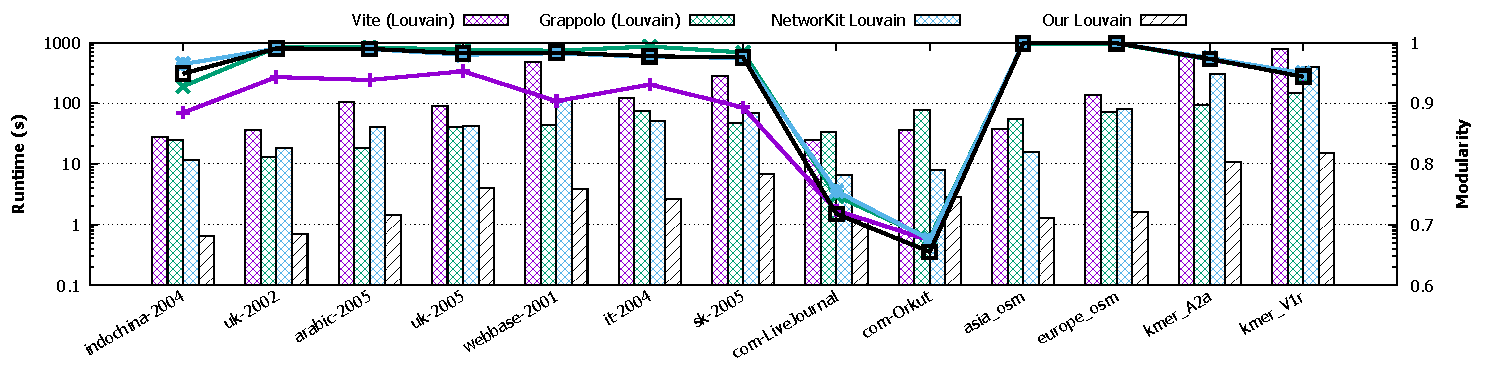
\includegraphics[width=0.98\linewidth]{out/louvain-compare.pdf}
  } \\[-2ex]
  \caption{Time taken (boxes), and modularity of communities obtained (lines) with \textit{Vite}, \textit{Grappolo}, \textit{NetworKit}, and our \textit{Louvain} for each graph in the dataset. Runtime is shown with logarithmic scale on the left Y-axis (in seconds), and modularity is shown with linear scale on the right Y-axis.}
  \label{fig:louvain-compare}
\end{figure*}

\begin{figure*}[hbtp]
  \centering
  \subfigure{
    \label{fig:louvain-compares--all}
    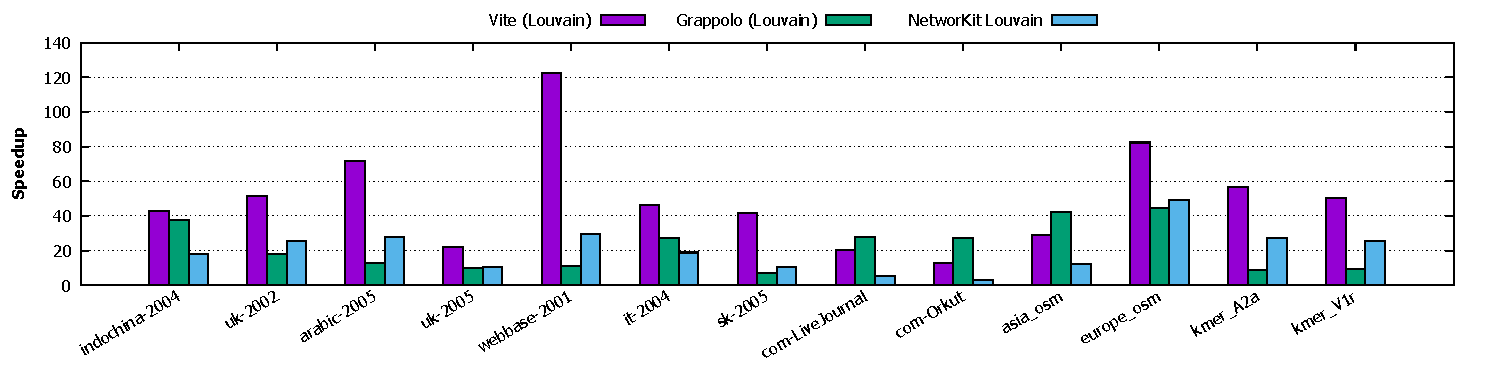
\includegraphics[width=0.98\linewidth]{out/louvain-compares.pdf}
  } \\[-2ex]
  \caption{Speedup of our \textit{Louvain} with respect to \textit{Vite}, \textit{Grappolo}, and \textit{NetworKit} for each graph in the dataset.}
  \label{fig:louvain-compares}
\end{figure*}

\begin{figure*}[hbtp]
  \centering
  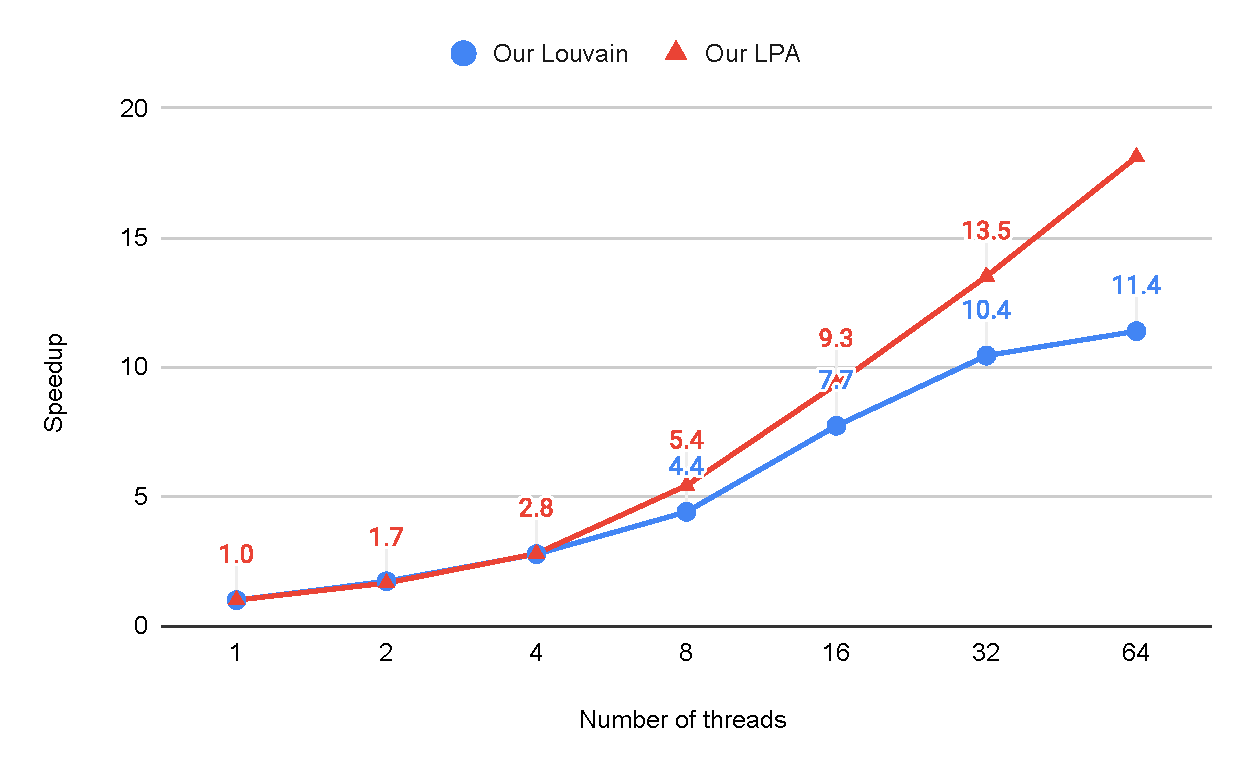
\includegraphics[width=0.68\linewidth]{out/louvain-ss.pdf} \\[-2ex]
  \caption{Speedup of our \textit{Louvain} with increasing number of threads.}
  \label{fig:louvain-ss}
\end{figure*}





\subsection{Comparing Performance of GVE-Louvain}

We now compare the performance of GVE-Louvain with Vite (Louvain), Grappolo (Louvain), and NetworKit Louvain. For Vite, we convert the graph datasets to Vite's binary graph format, run it on a single node (Vite supports distributed community detection) with threshold cycling/scaling optimization, and measure the reported average total time. For Grappolo, we measure the run it on the same system, and measure the reported total time. For NetworKit, we use a Python script to invoke \texttt{PLM} (Parallel Louvain Method), and measure the total time reported with \texttt{getTiming()}. For each graph, we measure the runtime of each implementation five times, for averaging. We also record the modularity of communities obtained, as reported by each implementation.

Figure \ref{fig:louvain-compare} shows the runtimes of Vite (Louvain), Grappolo (Louvain), NetworKit Louvain, and GVE-Louvain on each graph in the dataset. Figure \ref{fig:louvain-compares} shows the speedup of GVE-Louvain with respect to each implementation mentioned above. GVE-Louvain is on average $50\times$, $22\times$, and $20\times$ faster than Vite, Grappolo, and NetworKit respectively. On the \textit{sk-2005} graph, GVE-Louvain finds communities in $6.8$ seconds, and thus achieve a processing rate of $560$ million edges/s. Figure \ref{fig:louvain-compare} also shows the modularity of communities obtained with each implementation on the secondary (right) Y-axis. GVE-Louvain on average obtains $3.1\%$ higher modularity than Vite (especially on web graph), and $0.6\%$ lower modularity than Grappolo and NetworKit (especially on social networks with poor clustering).

\begin{figure*}[hbtp]
  \centering
  \subfigure{
    \label{fig:louvain-hardness--all}
    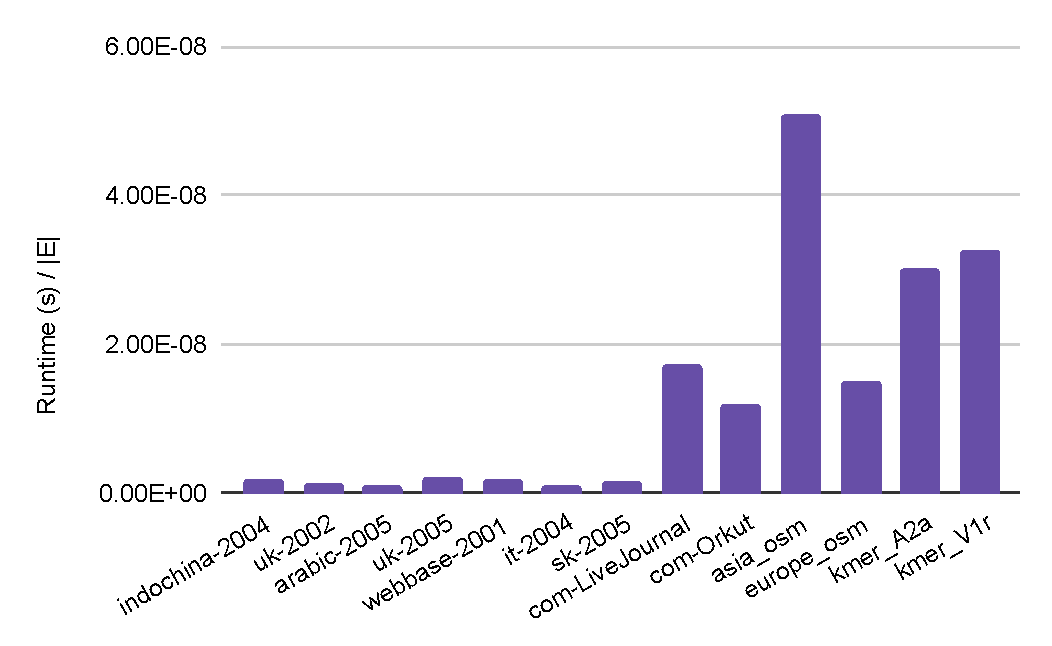
\includegraphics[width=0.48\linewidth]{out/louvain-hardness.pdf}
  } \\[-2ex]
  \caption{Runtime $/ |E|$ with our \textit{Louvain}, showing ...}
  \label{fig:louvain-hardness}
\end{figure*}

\begin{figure*}[hbtp]
  \centering
  \subfigure[Phase split]{
    \label{fig:louvain-splits--phase}
    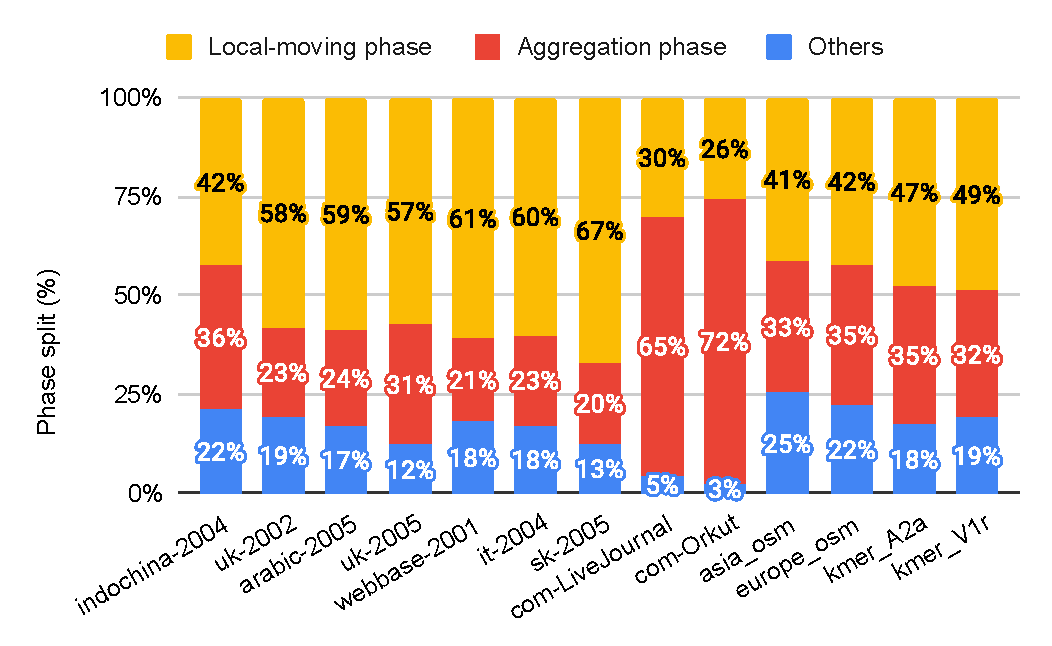
\includegraphics[width=0.48\linewidth]{out/louvain-phases.pdf}
  }
  \subfigure[Pass split]{
    \label{fig:louvain-splits--pass}
    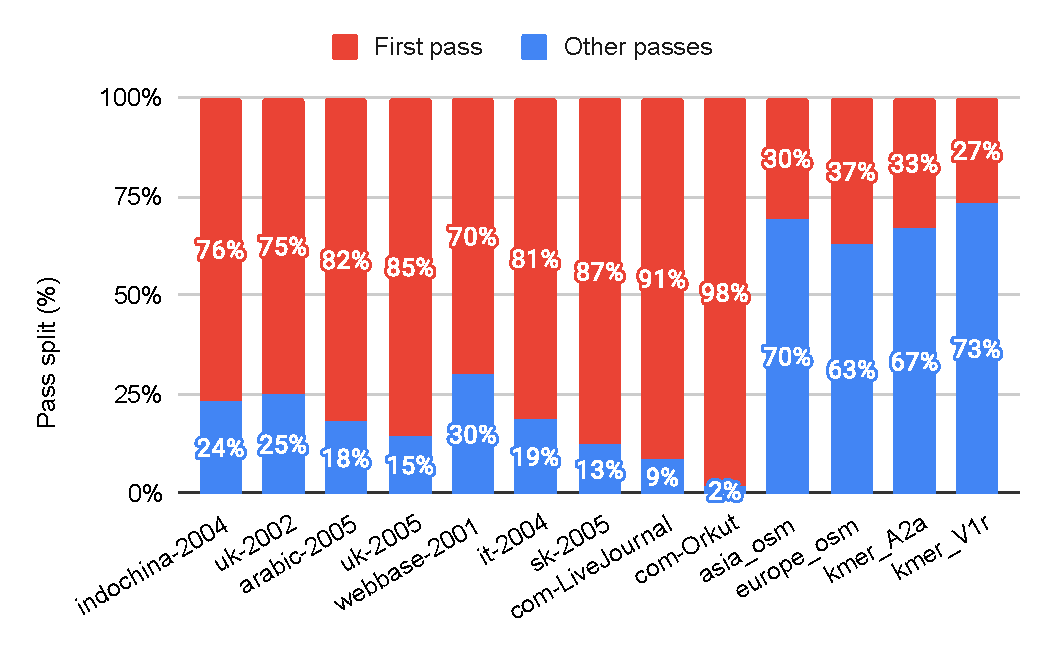
\includegraphics[width=0.48\linewidth]{out/louvain-passes.pdf}
  } \\[-2ex]
  \caption{Phase split of \textit{GVE-Louvain} shown on the left, and pass split shown on the right for each graph in the dataset.}
  \label{fig:louvain-splits}
\end{figure*}





\subsection{Results with our optimized implementation}

The combined optimizations yield impressive performance improvements in the OpenMP-based \StaLou{}, with a completion time of $6.8$ seconds on the \textit{sk-2005} graph containing $3.8 B$ edges (refer to Figure \ref{fig:louvainrak-sta}). We observe that graphs with lower average degree (\textit{road networks} and \textit{protein k-mer graphs}) and graphs with poor community structure (such as \verb|com-LiveJournal| and \verb|com-Orkut|) have a larger $\text{runtime}/|E|$ factor, as shown in Figure \ref{fig:louvainrak-hardness--louvain}.

The phase-wise and pass-wise split of the optimized \StaLou{} is shown in Figure \ref{fig:louvain-splits}. Note how $48\%$ (most) of the runtime of the algorithm is spent in the local-moving phase, while only $29\%$ of the runtime is spent in the aggregation phase of the algorithm. Further, $68\%$ (most) of the runtime is spent in the first pass of the algorithm, which is the most expensive pass due to the size of the original graph (later passes work on super-vertex graphs) \cite{com-wickramaarachchi14}.




\subsection{Strong Scaling of GVECD}

Finally, we measure the strong scaling performance of our Louvain and LPA. To this end, we adjust the number of thread from $1$ to $64$ in multiples of $2$ for each input graph, and measure the time taken for finding communities within each graph with our Louvain and LPA. As for each experiment above, for each graph, and for each thread count, we perform our Louvain and LPA five times for averaging. The results are shown in Figure \ref{fig:louvainrak-ss}. With 32 threads, finding communities with our Louvain obtains a $10.4\times$ speedup compared to running with a single thread, i.e., the performance of our Louvain increases by $1.6\times$ for every doubling of threads. Further, with 32 threads, finding communities with our LPA obtains a speedup of $13.5\times$ with respect to a single threaded execution, i.e., our LPA's performance increases by $1.7\times$ for every doubling of threads. Our LPA is thus more scalable than our Louvain due to its algorithmic simplicity (one only phase, in contrast to Louvain which has both a local-moving and an aggregation phase along with an expensive initialization step). At 64 threads, both our Louvain and our LPA are impacted by NUMA effects, and offer speedups of only $11.4\times$ and $18.1\times$ respectively. Note that our Louvain is significantly affected due to the reasons mentioned above.
